\chapter{Wstęp teoretyczny}
\label{cha:wstepTeoretyczny}

%---------------------------------------------------------------------------

\section{Procesy biznesowe}
\label{sec:procesyBiznesowe}

\subsection{Procesy biznesowe}
W każdym dużym przedsiębiorstwie, każdego dnia, wykonywana jest ogromna ilość czynności koniecznych do funkcjonowania tej organizacji. Ludzie oraz systemy podejmują najróżniejsze działania związane z różnymi, często nie mającymi wiele wspólnego zadaniami jak chociażby procesowanie płatności, składnie zamówień, wytwarzanie produktów czy ich transport. Przykłady te można mnożyć w zależności od sektora w jakim obraca się dana firma. Im jest ona większa, tym trudniej jest osobom zarządzającym zrozumieć i opisać poszczególne czynności. W pewnym momencie, kiedy ilość rożnych zadań rośnie do setek czy tysięcy staje się to niemożliwe i potrzebny jest sposób na zebranie wiedzy o pojedynczych operacjach i zamknięcie ich w uporządkowaną strukturę. Stąd narodził się pomysł na wykorzystanie wykorzystanie procesów biznesowych.

Procesy biznesowe opisują zbiór aktywność, które podejmuje grupa podmiotów w celu osiągnięcia celu biznesowego. W literaturze brakuje jednej ogólnie przyjętej definicji procesu biznesowego. W latach 90. XX wieku proponenci BPR, czyli Przeprojektowania procesów biznesowych (\textit{eng. Business process re-engineering}) starali się sprecyzować pojęcie procesu biznesowego. W książce ,,Process Innovation: Reengineering Work through Information Technology''\cite{davenport1993process} określono termin ten jako ,,Ustrukturyzowany, mierzalny zbiór działań, których celem jest wytworzenie określonego produktu dla określonego klienta lub rynku''. Autor położył nacisk na zbiór kroków prowadzących do celu, raczej niż na końcowy efekt. W dalszej części autor pisze ,,Proces jest zatem określonym uporządkowaniem czynności roboczych w czasie i przestrzeni, z początkiem i końcem oraz jasno określonymi wejściami i wyjściami: strukturą działania.''. Inni pionierzy BPR Michael Hammer i James Champy zaproponowali  podejście ,,Proces biznesowy to zbiór działań, który pobiera jeden lub więcej rodzajów danych wejściowych i tworzy wynik, który ma wartość dla klienta''\cite{HAMMER199390}. Autorzy dają większą dowolność, co do definicji procesu, nie wspominając o konieczności jego logicznej organizacji czy mierzalności. Z kolei Jacobson zupełnie pomija konieczność zamknięcia procesu w jakiekolwiek ramy: ,,Zestaw czynności wewnętrznych wykonywanych w celu obsługi klienta''\cite{JacobsonObjectAdvantage}. Nacisk na konieczność odniesienia procesów do wymiernych środków firmy widzimy w definicji: ,,Procesy biznesowe są aktywną częścią biznesu. Opisują funkcje firmy i obejmują zasoby, które są używane, przekształcane lub wytwarzane. Proces biznesowy to abstrakcja, która pokazuje współpracę między zasobami i transformację zasobów w biznesie. Podkreśla, w jaki sposób wykonywana jest praca, zamiast opisywać produkty lub usługi wynikające z tego procesu.''\cite{Eriksson2000BusinessMW}. Szczególnie ważny jest tutaj fragment o transformacji zasobów, gdyż każe on rozumieć poszczególne aktywności w procesie jako powiązane ze sobą i kończące się namacalnymi rezultatami. Definicja ,,Proces biznesowy to seria kroków mających na celu wytworzenie produktu lub usługi. W wyniku niektórych procesów produkt lub usługa jest odbierana przez zewnętrznego klienta organizacji. Nazywamy te podstawowe procesy. Inne procesy wytwarzają produkty, które są niewidoczne dla klienta zewnętrznego, ale są niezbędne do efektywnego zarządzania firmą. Nazywamy te procesy wsparcia''\cite{rummler_brache_1995} wprowadza rozgraniczenie na podtypy procesów. Ważnym jest jednak że nie jest koniecznością, aby rezultaty procesu były widoczne na zewnątrz organizacji. Warto też zaznaczyć, że procesy biznesowe nie dotyczą jednej osoby czy nawet działu, a raczej udział w nich bierze wiele ludzi, maszyn czy systemów z różnych działów połączonych celem dostarczenia wspólnej wartości biznesowej.

Powyższe definicji skupiają się na delikatnie odmiennych aspektach procesów biznesowych, nie zawsze szczegółowo wspominając o innych. Starając się usystematyzować powyższe sformułowania, chcąc zbudować bazę do dalszej analizy tematu, można przyjąć, że procesy biznesowe charakteryzują:
\begin{itemize}
  \item[•] Określony cel, którym jest wytworzenie wartości dla klienta zewnętrznego lub pośrednio firmy - klienta wewnętrznego. Jednak warto jeszcze raz zaznaczyć ze proces biznesowy skupia się na sposobie osiągnięcia celu, a nie opisie celu samego w sobie. 
  \item[•] Dyskretny, jasno zdefiniowany i identyfikowalny zbiór aktywności. 
  \item[•] Jasno określony początek - wejście i koniec - wyjście.
  \item[•] Zależność przyczynowo-skutkowa pomiędzy kolejnymi procesami.
\end{itemize}

Żeby lepiej zilustrować czym jest proces biznesowy, poniżej znajduje się prosty przykład często spotykanego procesu. Oczywiście, prawdziwy proces będzie składał się z o wiele większej liczby aktywności.

\begin{figure}[h]
	\centering{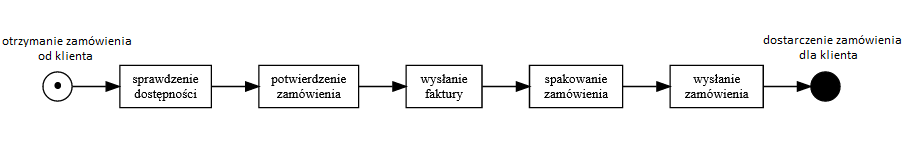
\includegraphics[scale=0.7]{simple-business-process.png}}
	\caption{\label{fig:simple_business_process}Przykład prostego procesu}
\end{figure}

Zauważmy, że mamy jasno zdefiniowany wejście - otrzymanie zamówienia od klienta oraz wyjście, kiedy dostarczamy oczekiwaną wartość dla klienta, a całość składa się z serii tworzących logiczną całość aktywności. Aktywności są konkretnie zdefiniowane. Standardem jest definiowanie aktywności w formie równoważników zdań.


\subsection{Zarządzanie procesami biznesowymi}
Zdefiniowanie proces biznesowego otwiera wiele możliwości analizy działań przedsiębiorstwa i w skutek tego wprowadzanie usprawnień. Dziedziną, która się tym zajmuje jest zarządzanie procesami biznesowymi (\textit{eng. Business process modeling}) zwane w skrócie BPM. Sercem jest proces, a samo BPM jest dyscypliną używającą różne metody, technik i sposobów w celu projektowania, wprowadzania w życie, zarządzania i analizy procesów biznesowych \cite{BPMDemystified}. 

Celem stosowania metod zarządzanie procesami biznesowym jest udoskonalanie procesów w danej organizacji biznesowej. Udoskonalanie może być rozumiane jako w różnoraki sposób w zależności od kierunku rozwoju firmy. Może to być na przykład redukcja czasu, kosztów, czy dostarczanie lepszego produktu końcowy. Ważnym jest aby było to podejście całościowe i odnosiło się do całego zbioru aktywności w ramach danego procesu. Usprawnianie pojedynczej aktywności to nie BPM. Patrząc na przykład powyżej, jeśli wprowadzilibyśmy usprawnienia w ramach wysyłania faktury, robiąc to elektronicznie zamiast tradycyjną poczta, mimo że taka zmiana przyniosłaby poprawę wydajności, nie mielibyśmy do czynienia z zarządzaniem procesami biznesowymi. O BPM moglibyśmy mówić, gdybyśmy  znaleźli sposób, żeby przeprojektować cały proces tak, żeby wysyłanie faktury nie było potrzebne lub odwrotnie, jeśli dodalibyśmy nowe aktywność, która usprawniłaby proces jako całość czy nawet zmieli kolejności zdań w procesie, gdyż zmiany w ramach poszczególnych, jednostkowych aktywności nie są konieczne, żeby ulepszyć proces jako całość \cite{BPMWhat}.

Zarządzanie procesami biznesowymi jest zbiorem praktyk, działań mających na celu udoskonalanie procesów. Trzeba więc rozumieć BPM jako pojęcie abstrakcyjne, jednak szczególnie w dzisiejszym świecie, zarządzanie procesów biznesowych nie może się obyć bez wsparcia ze oprogramowania czy technik znanych z różnych dziedzin informatyki \cite{BPMSurvey}. Na lepsze zrozumienie czym zajmuje się zarządzanie procesami biznesowymi oraz w jaki sposób możemy zastosować informatykę, a w szczególności eksplorację procesów w tej dziedzinie, może pozwolić definicja cyklu życia procesu biznesowego.

\begin{figure}[h]
	\centering{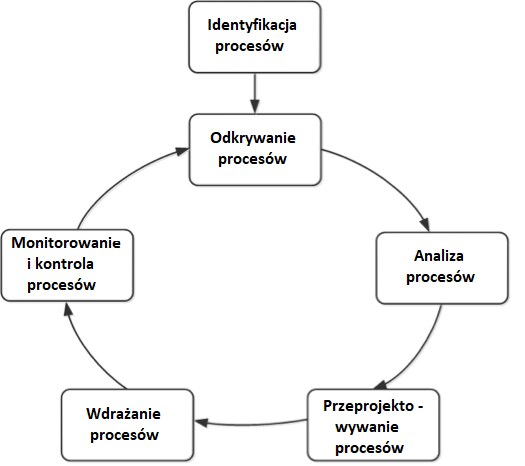
\includegraphics[scale=0.55]{lifecycle.png}}
	\caption{\label{fig:lifecycle}Cykl życia procesu biznesowego}
\end{figure}

Cykl życia procesu biznesowego (\textit{eng. Business process lifecycle}) przedstawiono na rys. \ref{fig:lifecycle} \cite{dumas2013fundamentals}. Jest to zbiór kroków niezbędnych do skutecznego zarządzania procesami biznesowymi. W celu dostosowania do zmieniającej się rzeczywistości, poszczególne kroki powinny być co pewien czas powtarzane. 

Konieczność powtarzania elementów cyklu życia procesu biznesowego sygnalizuje przewagę komputerów i algorytmów    nad wykonywanie tych operacji przez człowieka. Metody informatyczne są stosowane, na każdym z wymienionych etapów. W szczególności dane zebrane w wyniku monitorowania procesów dają nam możliwość zastosowania metod z zakresu eksploracji procesów (sekcja \ref{sec:eksploracja}). Praca skupia się w głównej mierze na odkrywaniu procesów, czyli znajdowaniu istniejących już procesów na podstawie realny danych. Należy zaznaczyć, że identyfikacja polega na ogólnym rozpoznaniu i nazwaniu zachodzących procesów, podczas gdy odkrywanie jest bardziej szczegółowe, a w jego wyniku otrzymujemy dokładny model.  

%---------------------------------------------------------------------------

\section{Eksploracja procesów}
\label{sec:eksploracja}
\subsection{Modelowanie procesów biznesowych}
Na rys. \ref{fig:simple_business_process} przedstawiono przykład uproszczonego procesu biznesowego. Łatwo sobie wyobrazić, że proces ten w rzeczywistości może być znacznie bardziej skomplikowany. Część aktywności może być wykonywana równolegle, niektóre zdarzenia w ogóle nie zaistnieją lub będą występować kilkukrotnie w ramach jednego procesu. 


W sytuacji, w której zamówiony przez klienta towar będzie niedostępny, logiczne wydaje się poinformowanie go o opóźnieniu oraz danie mu możliwości anulowanie zamówienia lub jego kontynuacja i ponowne sprawdzenie dostępności. Ponadto, czynności takie jak wysłanie faktury oraz spakowanie i wysłanie zamówienia mogą być wykonane w dowolnej kolejności czy nawet jednocześnie przez dwie różne osoby. Proces staje się bardziej skomplikowany i konieczna do stworzenia jego modelu jest bardziej złożona notacja niż użyta do przedstawienia prostego procesu. 
Istnieje wiele notacji do modelowania procesów biznesowych, wśród nich można wymienić schematy blokowe, diagramy aktywności UML, łańcuchy procesu sterowanego zdarzeniami (\textit{eng. Event-driven Process Chains}), sieci Petriego \cite{BPMComparission}. Modelując procesy biznesowe warto korzystać z 
Obecnie najpopularniejszą notacją używaną do opisu procesów biznesowych jest Business Process Modeling Notation, w skrócie BPMN \cite{omg2011bpmn}. Daje ona możliwość opisania w jednoznaczny sposób skomplikowanych procesów czy stworzenia diagramów współdziałania procesów, jednocześnie pozostając łatwą do zrozumienia.

Na grafice poniżej przedstawiono notację opartą o elementy BPMN, używaną w dalszej części pracy. Składają się na nią zdarzenia początkowe i końcowe, połączenia, bramki logiczne oraz aktywności, gdzie czarnym kwadratem oznaczono sytuację, w której żadna aktywność nie jest wykonywana, możliwe tylko w bramce LUB. 
\clearpage
\begin{figure}[h]
	\centering{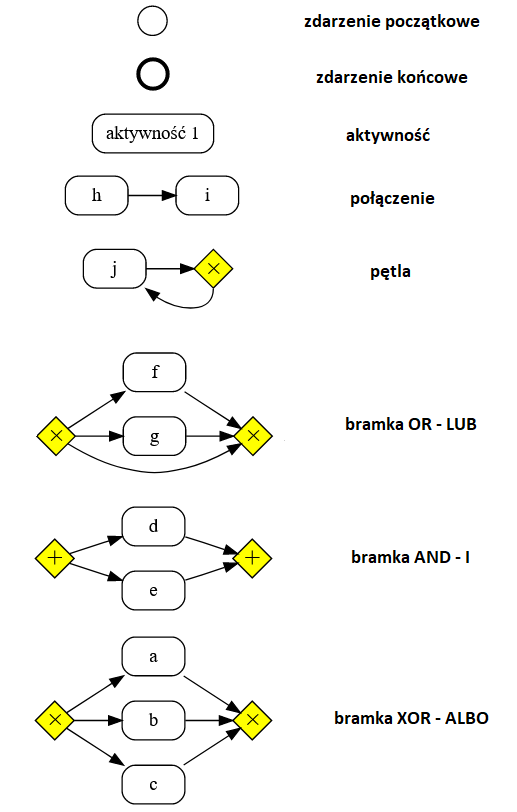
\includegraphics[scale=0.41]{BPMNelements.png}}
	\caption{\label{fig:bpmn_example}Elementy BPMN}
	\label{fig:lifecycle}
\end{figure}

Korzystając z tej notacji, można przedstawić opisany wcześniej proces. Na rys.  \ref{fig:complicated_business_process_1} widać model po modyfikacjach. 

\begin{figure}[h]
	\centering{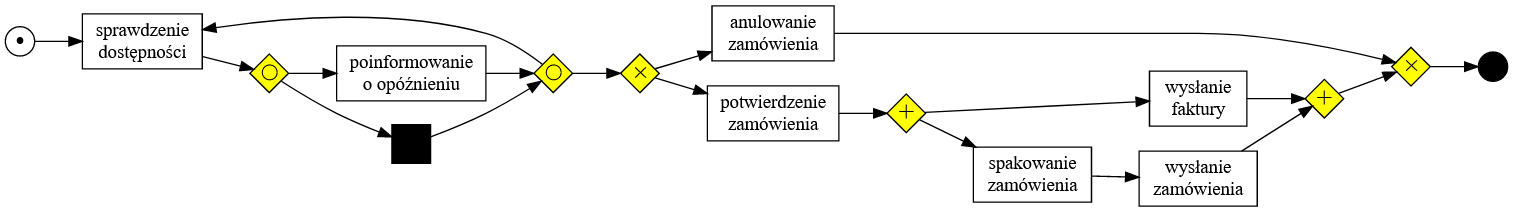
\includegraphics[scale=0.3]{complicated-process-example-1.png}}
	\caption{\label{fig:complicated_business_process_1}Rozbudowany procesu - przykład 1}
\end{figure}

Możliwe jest teraz poinformowanie klienta o opóźnieniu, a następnie anulowanie zamówienia lub powtórne sprawdzenie dostępności. Model ten jednak nie jest wystarczająco precyzyjny i pozwala na potwierdzenie zamówienia po informacji o jego opóźnieniu, a bez uprzedniego ponownego sprawdzenia dostępności. Można zaproponować inny model (rys. \ref{fig:complicated_business_process_2}), który rozwiązuje powyższe problemy, jednak aktywność - poinformowanie o opóźnieniu - występuje na nim dwukrotnie, co jest niepożądane i  pogarsza jego czytelność.

\begin{figure}[h]
	\centering{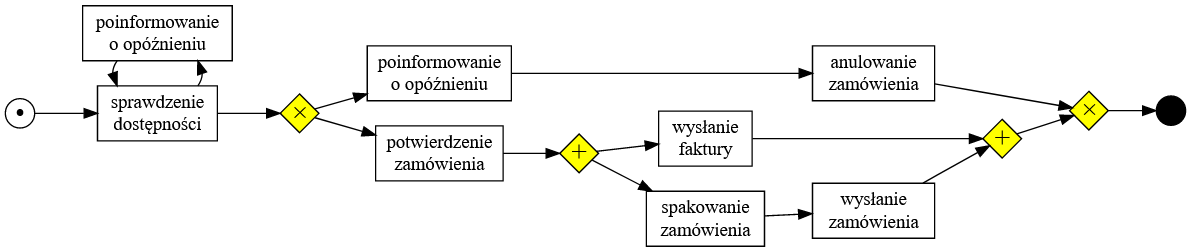
\includegraphics[scale=0.35]{complicated-process-example-2.png}}
	\caption{\label{fig:complicated_business_process_2}Rozbudowany procesu - przykład 2}
\end{figure}

Ponadto, w pewnych przypadkach klient może mieć możliwość rezygnacji z zamówienia bez ówczesnego informowania go o opóźnieniu, a z czego nie zdawano sobie sprawy, wtedy konieczne może być stworzenie zupełnie innego modelu. Aby radzić sobie z tymi problemami powstał szereg zestawów wytycznych, którymi warto się kierować modelując procesy biznesowe. Wśród takich zasad można wymienić: zminimalizuj liczbę elementów w modelu, zminimalizuj liczbę ścieżek w modelu, używaj jednego zdarzenia początkowego i jednego końcowego, unikaj bramek LUB - OR , zdekomponuj model zawierający więcej niż 50 elementów \cite{7PMG}.

Modelowania procesów biznesowych jest próbą stworzenia uproszonej wersji rzeczywistości na podstawie przewidywań i założeń. Modele dają abstrakcję, użyteczne przybliżenie rzeczywistości, jednak należy pamiętać, że ,,Wszystkie modele są błędne'' i rzeczywisty proces najprawdopodobniej będzie różnił się od nawet najlepszego modelu. 


\subsection{Eksploracja procesów}

W dzisiejszych czasach standardem jest, ze organizacje biznesowe korzystają z systemów informatycznych, takich jak chociażby systemy ERP czy CRM wspierających ich działalność. Systemy te rejestrują dane o procesach, które wspierają. Dane te mogą być później analizowane i wykorzystane do wprowadzenie usprawnień w działaniu firmy.   

Rozumieją, że tradycyjne metody są wolne, a konieczność ich ciągłego powtarzania, połączone z wszechobecnym trendem automatyzacji obecnym w biznesie sprawiają, że eksploracja procesów zyskuje na znaczeniu \cite{GARTNER}. Ważna jest możliwość szybkiej adaptacji do zmian, automatyzacja pozwala na wykonywanie powtarzalny zmian i ograniczenia błędów.

Jest to szeroko pojęta dziadzina, która zawiera różne aplikacje metoda informatyki do procesów. 
Jest wartościowym dodatkiem do innych metod eksploracji danych, gdyż daje pełniejszy obraz zamiast skupiać się pojedynczym rezultacie końcowym i tworzyć predykcje, celem jest zrozumienie całej procesu i akcji, które prowadzą do końcowego rezultatu. Jest ot trudniejsze, ale jakże cenne z punktu widzenia biznesowego, gdyż jakakolwiek zmiana w trakcie procesu może sprawić, że przewidywania będą kompletnie trafione, a zrozumienie całego procesu pozwala na pełniejszy obraz i łatwiejsze dostosowanie do zmian. 

Ponadto, procesy biznesowe są często rozumiane przez analityków i metoda na łatwe odniesienie się do oczekiwań biznesowych i stworzenie ścisłych, powtarzalnych i sprawdzalnych ram na dziedzinie, która w więkości opierała się na czarenej magii, bullshicie i coacgingowy bredniach jest nadwyraz cenne. Eksploracja procesów biznesowych oparta jest na danych i nie ma w niej dużo miejsca na przypuszczenia i domysły.

tu by wypdalo krotki opis techniczny
Wyróżnia 3 podkategorie \cite{mining-overview}: 
\begin{itemize}
  \item[•] automatyczne odkrywanie procesów
  \item[•] sprawdzanie zgodności (\textit{eng. conformance checking})
  \item[•] udoskonalanie procesu (\textit{eng. performance mining})
\end{itemize}


\subsection{Dzienniki zdarzeń}

Danymi wejściowymi dla algorytmów z dziedziny eksploracji procesów są dzienniki zdarzeń.
 
\begin{figure}[h]
	\centering{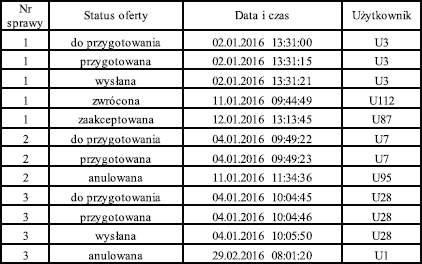
\includegraphics[scale=0.8]{event-log.png}}
	\caption{\label{fig:event_log_example}Przykład dziennika zdarzeń}
\end{figure}

W kontekście odkrywania procesów biznesowych ważne są dla nas tylko zdarzenia i kolejność ich wykonywania.
Przyjmuje się, że aby mówić o dzienniku zdarzeń powinien on zawierać 3 informacje: numer przypadku, czyli unikalny identyfikator zbioru aktywności, nazwę poszczególnych aktywności oraz datę jej wykonania - ważną tylko w kontekście kolejności wykonywania pojedynczych aktywności. Ponadto może on zawiera inne zbędne w kontekście odkrywania procesów biznesowych dodatkowa informacje, takie jak: podmiot wykonującym daną aktywność, miejsce, koszt czy aktualny postęp wykonania. Oczywiście te pozostałe dane mogą być wykorzystywane w kolejnych etapach analizy i usprawniania procesu.

Mając do dyspozycji te 3 informacje - poszczególne przypadki, aktywności na nie się składające oraz ich kolejność, zliczamy jak często poszczególne aktywności występują w danej kolejności. Każdy tak przypadek zwany jest wariantem. Ponadto musimy wiedzieć jak często dany wariant wystąpił.

\begin{figure}[h]
	\centering{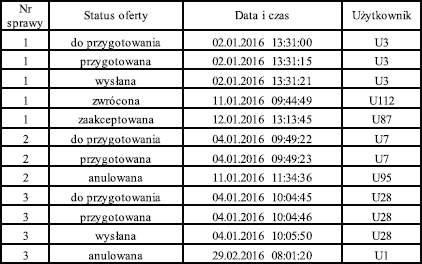
\includegraphics[scale=0.8]{event-log.png}}
	\caption{\label{fig:process_variants_example}Przykład wariantów procesu}
\end{figure}

Dla poprawy czytelności aktywność często reprezentowane są jako symbole, np. kolejne litery alfabetu, zamiast pełnej nazwy.

\subsection{Automatyczne odkrywanie procesów biznesowych}

Directly-flows-graphs.
Automatyczne odkrywanie procesów biznesowy jest podgrupą i obejmuję techniki przekształcania danych w procesy. Ważne, że proces już istnieje, a my tylko go odkrywamy. Wejściem jest dziennik zdarzeń.
Procesy zaprojektowane nie zawsze są realizowane w praktyce. Ważne jest, żeby proces był oparte tam analizie prawdziwych danych, a nie spekulacjach i założeniach. Pozwala na znajdowanie procesu takim jaki jest, a nie takim jakim chcianoby, żeby  był.


4 kroki, żeby odkrywac proces

\begin{figure}[h]
	\centering{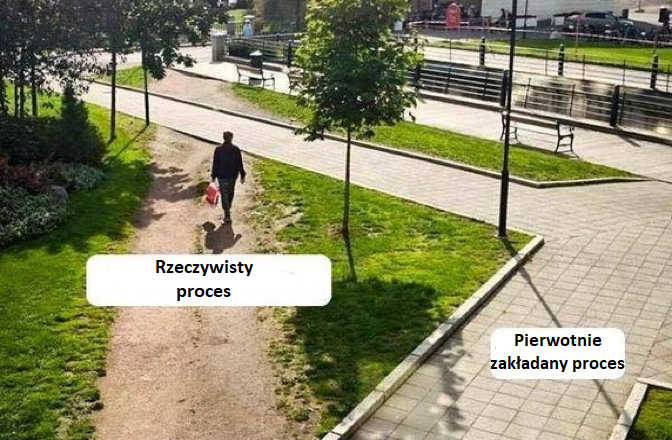
\includegraphics[scale=0.5]{model-vs-real.png}}
	\caption{\label{fig:subcaption_example}Proces rzeczywisty i pierwotnie zakładany}
\end{figure}

Klasyczne algorytmy do wykrywania procesów biznesowych:
\begin{itemize}
  \item[•] Alpha algorithm
  \item[•] The ILP Miner
  \item[•] Heuristic Miner 
  \item[•] Multi-phase Miner
  heuristics, structured
\end{itemize}

Metryki opis ogólny


Zalety algorytmów genetycznych 


%---------------------------------------------------------------------------

\section{Metryki}
\label{sec:metryki}
\cite{doi:10.1142/S0218843014400012}
\subsection{Metryki a fitness function}
\subsection{Prostota}
Najprostsza z metryk. \newline
$M_{pro} = 1 - \frac{ilosc\ duplikatow\ w\ modelu\ +\ ilosc\ brakujacych\ wartosci\ w\ modelu}{ilosc\ unikalnych\ zdarzen\ w\ logu\ +\ ilosc\ zdarzen\ w\ modelu}$
\subsection{Odwzorowanie}
Jest to najbardziej kosztowna obliczeniowo metryka. Pozostałe metryki obliczane są na podstawie tej metryki. \newline
$M_o = (1 - \sum_{0}^{ilosc\ procesow\ w\ logu} \frac{blad\ odwzorowania\ logu\ w\ modelu}{minimalna\ długosc\ sciezki\ w\ modelu\ +\ długosc\ sciezki\ w\ logu})^4$

Przykład liczenia odwzorowania: \newline

\subsection{Precyzja}
Unikanie underfittingu \newline
$M_{pre} = (1 - \sum_{0}^{ilosc\ zdarzen\ w\ modelu} \frac{ilosc\ osiagalnych\ zdarzen\ w\ modelu - ilosc\ osiagalnych\ zdarzen\ w\ logu}{ilosc\ osiagalnych\ zdarzen\ w\ modelu})^{\frac{1}{3}} $
\subsection{Generalizacja}
Unikanie overfittingu \newline
$M_g = \frac{1 - \sum_{0}^{ilosc\ zdarzen\ w\ logu} \frac{1}{\sqrt{ilosc\ wystapien\ zdarzenia}}}{ilosc\ zdarzen\ w\ logu} $
\subsection{Złożoność}
POET
Promuje rozwiązywanie prostych problemów w prosty sposób \newline
$M_z = 1 - \frac{1}{\sqrt{1 - odwzorowanie\ *\ \sqrt{zlozonosc\ modelu}}} $


%---------------------------------------------------------------------------

\section{Ewolucja genetyczna}
\label{sec:ewolucjaGenetyczne}
\subsection{Algorytmy genetyczne}
\cite{ryan_collins_neill_1998}
Algorytmy genetyczne są inspirowaną selekcją naturalną  heurystyką, która używa znanych z ewolucji biologicznej operacji jak mutacja, selekcja czy krzyżowanie do rozwiązywania problemów wyszukiwania i optymizacji. Ich ideą jest zaproponowanie metody przeszukiwania przestrzeni losowy rozwiązań w celu wyszukania najlepszych z nich. Pierwszy raz zostały zaproponowane w \cite{10.5555/138936}.

Sposób działania algorytmów genetyczny polega na stworzeniu populacji losowych rozwiązań zwanych genotypami lub chromosomami, które kodowane są za pomocą licz całkowitych i zapisywane ww tablicy jednowymiarowej. Następnie dla każdego elementu populacji obliczane są metryki pozwalające ocenić jak dobre jest wygenerowane rozwiązanie. Po sklasyfikowaniu rozwiązań generujemy nową populację mutując lub krzyżując głownie choć nie tylko najlepsze chromosomy. Proces ten jest powtarzany do momentu otrzymania satysfakcjonującego rozwiązania.  

Selekcja:
Selekcja proporcjonalna - wybieramy losowo rozwiązania z puli wszystkich rozwiązań z warunkiem, że rozwiązania z największą wartością metryk mają największą szansę na bycie zachowanymi w populacji. Jest to najpopularniejsza metoda selekcji i najczęściej umożliwiająca najszybsze znalezienie rozwiązania. Pozwala na elityzm, czyli zachowanie części najlepszych genotypów w przyszłej populacji.

Selekcja turniejowa - wybieramy podzbiór ze zbioru rozwiązań i zachowujemy w przyszłej najlepsze rozwiązanie z tego podzbioru.
Rozwiązanie to pozwala na duży wpływ na presję genetyczną - zwiększając wielkość podzbioru ograniczamy szansę na wybór z niską wartością metryk.  Jest to także metoda, która łatwe zrównoleglenie.

Krzyżowanie - :
Krzyżowanie punktowe - spośród dwóch genotypów losowo wybieramy jeden punkt, następnie tworzymy dwa nowe genotypy pierwszy z chromosomów na prawo od punktu w pierwszym genotypie i na lewo w genotypie drugim oraz drugi z dwóch pozostałych.

Krzyżowanie dwupunktowe - spośród dwóch genotypów losowo wybieramy dwa punkty, następnie część pomiędzy tymi punktami jest zamieniana pomiędzy genotypami.

Krzyżowanie n-punktowe - uogólnienie powyższych krzyżowań dla n punktów.

Krzyżowanie zamiana w drzewie - genotyp może być reprezentowany jako drzewo, w tej metodzie zamieniamy ze sobą dwa poddrzewa, tworzone są tylko prawidłowe rozwiązania, jednak jest to metoda wymagająca większej ilości obliczeń. 


Mutacja:
Mutacja punkowa - dowolna wartość w tablicy zostaje zmieniona na inną losową wartość. Pozostałe produkcje pozostają niezmienione.

Mutacja zamiana w drzewie - genotyp może być reprezentowany jako drzewo, w tej metodzie tworzone jest nowe poddrzewo, przy tej metodzie tworzone są tylko prawidłowe rozwiązania, jednak jest to metoda wymagająca większej ilości obliczeń. 

 
  
\subsection{Ewolucja genetyczna a inne algorytmy uczenia maszynowego}
Algorytmy genetyczne pozwalają przeszukać najszerszą przestrzeń rozwiązań. Pozwalają na znajdowanie nieoczywistych rozwiązań.  
Inna heurystyką, która używa losowo rozwiązuje problem jest simulated annealing. Algorytm genetyczny jest łatwy w zrównogleniu i pozwala znaleźć globalne rozwiązanie.
Sieci neuronewe:
Pula rozwiązań zamiast jednego rozwiązywania. Szersze przeszukiwanie rozwiązań. 

Obejrzeć filmik na mlst.
\subsection{Ewolucja gramatyczna}
Ewoluuje gramatykę za pomocą metod ewolucji genetycznej w celu znalezienia programu, który najlepiej rozwiązuje problem.
Podejście to zostało zaproponowane w \cite{ryan_collins_neill_1998}. 

%---------------------------------------------------------------------------

\section{Gramatyka}
\label{sec:gramatyka}
\subsection{BNF}
Backus-Naur from jest notacją używaną do kodowaniu gramatyk bezkontekstowych.

Gramatyka bezkontekstowa - 

Gramtyka G=(N,$\Sigma$,P,S) - 

\subsection{Tworzenie gramatyki pod kątem ewolucji}

W celu ograniczenia niepotrzebnych obliczeń gramatyka powinna tworzyć jak najmniej niewłaściwych rozwiązań. 
Tworząc gramatykę pod kątem wykorzystania jej w procesie ewolucji ważne jest, żeby ilość produkcji jak najlepiej odzwierciedlała jak często chcemy uzyskać dany stan.
Stosując operator mutacji możemy uzyskać genotypy, które nie należą do języka, czyli nie są właściwym rozwiązaniami. Żeby ograniczyć zbędne obliczenia gramatyka powinna minimalizować szansę na to, że zamieniając produkcję na dowolną inną dostępną dla danego symbolu produkcję uzyskamy słowo które nie należy do języka.
Przykład:
a+b
<e> = aSe | b
<S> = + | -

<e> = aee | b | + | -

Produkcja 1:

<e> -> aSe -> a+e -> a+b
Produkcja 2:
<e> -> aee -> a+e -> a+b

Jeśli w kroku a+e zajdzie mutacja, może uzyskać gramatykę np. a+-, która nie należy do języka, dlatego pierwsza gramatyka jest lepsza.